%%%%%%%%%%%%%%%%%%%%%%%%%%%%%%%%%%%%%%%%%%%%%%%%%%%%%%%
\chapter{オガワかをり\index{おがわかおり@オガワかをり}}
\label{chap:Kawori}
%%%%%%%%%%%%%%%%%%%%%%%%%%%%%%%%%%%%%%%%%%%%%%%%%%%%%%%

なぜか知らんが、度々、重症患者たちからの絶大な人気を誇るオガワかをり\index{おがわかおり@オガワかをり}。本章ではこの人物について、今一度振り返ってみる。


\section{かをり\index{かをり@かをり}という概念}
世の中には、様々な概念\index{がいねん@概念}が存在する。しかし、その概念\index{がいねん@概念}の範疇を越えようとしている概念が存在する。それこそまさに「かをり\index{かをり@かをり}」である。その概念\index{がいねん@概念}について詳しく述べる。

\subsection{爆誕}
 かをりという概念\index{がいねん@概念}が爆誕したのは1964年の12月25日である。奇しくもこの日は、あの伝説のアーティスト、オガワインティライミ\index{おがわいんてぃらいみ@オガワインティライミ}氏が生まれた日である6月24日から半年という、奇跡である。その上で、爆誕した日がクリスマスという、もはやイエスキリストという概念との比較すべき存在であることがわかる。\\
 ここで、LBFという存在を紹介する。LBF(University Bible Fellowship)とは大学生聖書読み宣協会のことで、なんか知らんけど謎の団体である。この団体の概念\index{がいねん@概念}はさておき、図\ref{ubf}を見ていただきたい。ここでは、コリント人への手紙が記されており、この「98-2講 私たちはキリストのかおり」には明確に「私達はキリストのかおり」と記してあるのである。念のため、この本文の一部を以下に示す。\\

\shadowbox{
\begin{tabular}{l}
98-2講 私達はキリストのかおり\\
 \\
投稿者: Jubfadmin 掲載日: 2004/12/23 (4352 回閲覧)\\
1998年コリント人への手紙第二 第2講\\
私達はキリストのかおり\\
 \\
御言葉:コリント人への手紙第二2:1?17\\
 \\
要 節:コリント人への手紙第二2:15\\
 \\
「私たちは、救われる人々の中でも、滅びる人々の中でも、神の前にかぐわしいキリストの\\
かおりなのです。」\\
今日の御言葉はクリスチャンの影響力に関する御言葉です。私達がどうすれば良い影響力を\\
及ぼすクリスチャンになれるでしょうか。今日の御言葉を通してその秘訣を学ぶことができる\\ように祈ります。\\
 \\
?。あふれるばかりの愛(1?11)\\
 第一に、涙の人、パウロ(1?4)。1節をご覧下さい。「そこで私は、あなたがたを悲し\\
ませることになるような訪問は二度とくり返すまいと決心したのです。」使徒パウロがコリント\\
教会を開拓して離れている間にコリント教会は分裂して党派に分かれ、パウロの権威を認めない\\
人達がいました。そのためにパウロは急いでコリント教会を訪問しましたが、事態は改善される\\
どころかますます悪化し、さすがのパウロも、悲しみを残して帰って来ました。それでパウロは彼\\
らを悲しませることになるような訪問は二度と繰り返すまいと決心しました。そのような状況では、\\
たとえ訪問しても、パウロもコリント人もお互いに悲しい思いをさせられるばかりだったからです。
\end{tabular}
}\\
 \\
 まず問題なのが、このコリント人への手紙が98-2まであるということである。長すぎるのである。しかも文字化けしているのである。カスカスカス\index{かす@カス}。そして、極めつけは「私達はキリストのかおり」という文章である。キリストという概念に対して「私達」という複数形の表現から、複数人の概念であることが推測される。そのくせに、キリストのかおりという概念に収束するのである。しかし、ここで注目したいのは「かおり」という表記である。我々が提示する概念は「かをり」であるため、このキリストのかおりはあくまで下位互換であり、手下であり、不完全体である。ここから完全なキリストのかをりになるべく、懸命な努力をしていくのである。\\

\begin{figure}[H]
  \centering
  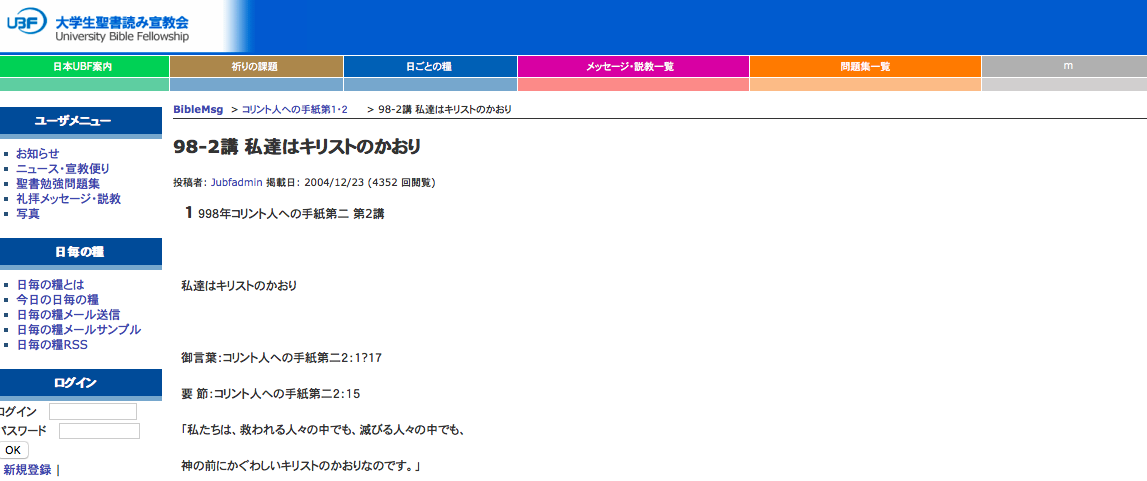
\includegraphics[clip,scale=0.4]{./section/Kawori/figures/ufb.png}
  \caption{投稿者: Jubfadmin 掲載日: 2004/12/23 (4352 回閲覧)}
\label{ufb}
\end{figure}

\subsection{世界デビュー}
ここからは、かをり\index{かをり@かをり}がかをりたる所以である。その存在が世界に明るみになった、デビューという概念が存在する。\\
事件が起こったのは2015年である。オガワインティライミ氏\index{おがわいんてぃらいみ@オガワインティライミ}が研究室にて爆誕した当初、その研究室ライフを謳歌すべく、自撮り棒の購入を試みた。どうせなら、公での購入であるため、研究室のパソコンを使用してAmazonを利用しようとした。図\ref{jidoribou}は当時、購入しようとした自撮り棒を同様のもののスクショを示す。

\begin{figure}[H]
  \centering
  
\includegraphics[clip,scale=0.4]{./section/Kawori/figures/jidoribou}
  \caption{値段は当時と変わらず500円という驚異的な安さである。また、自撮り棒の取っ手の部分がゴム製のカバーが付いており、写真などを撮るときにボタンを押す際にズレてなかなか撮影がうまくいかず、放送ジーコ監督就任のお知らせ\index{ほうそうじーこかんとくしゅうにんのおしらせ@放送ジーコ監督就任のお知らせ}である。}
\label{jidoribou}
\end{figure}

この破格的な値段から、即購入が決定したのだが、送り先を研究室にするために、発送先の設定をしようとしたところ、事件は起きたのである。購入手続きの流れで、宛先としてあの存在が表示されたのである。\\

\shadowbox{
\begin{tabular}{c}
オガワかをり
\end{tabular}
}

まさに、概念が概念を超えた瞬間である。この奇跡的な現象を観測したのは、世界を股にかける精鋭の研究部隊のメンバーであるタケダ氏\index{たけだ@タケダ}とグバ氏とオバ氏である。最新の記憶の呼び起こし研究の結果によると、その場にいたのがタケダ氏とグバ氏\index{ぐば@グバ}とオバ氏\index{おば@オバ}であるという。彼らによって、このオガワかをり現象は瞬く間に世界中に広まり、これが伝説的な世界デビューとなった。その後というものの、度々、風の噂でその伝説が誕生していき、その存在についてより活発な研究が進むこととなった。また、その存在を肉眼で一目見ようと、命知らずの重症患者\index{じゅうしょうかんじゃ@重症患者}達が死闘を繰り広げていくのである。






\section{周りからの総評}
オガワかをり(通称、かをり)爆誕という概念は、時をかける少女の様に2015年以来、
常に我々の頭の中を支配してきた概念である。
急激に爆誕した、そのかをりという概念について多角的に考察しようと思う。
前節で議論したように、カヲリという概念は天から一瞬にして降り注いだ概念であり、爆発的なその急成長のスペードから、どの時点で発生したかという定義が非常に困難である。
明らかにAmazonでの買い物の段階で発生したのであるが、ここで今一度入学式からのカヲリ概念時間発展を追ってみたいと思う。
\par
この章ではまず我々の入学式の時点から卒業式にかけてどのようにカヲリという概念が時間発展したかを、時系列に沿って議論する。
また、卒業式では実際に我々が追い求めていたオガワカヲリと対面することになるのであるが、それらの決定的瞬間についても報告する。
そしてそれらの結論として、カヲリがいかに皆から愛されている女性であるかを示そう。

\subsection{入学式}

まず、入学式時点のおける集合写真を図\ref{fig:H24Nyugakushiki}示そう
\footnote{併せて抑えて起きたいこの時点で形成された概念として、有名なファンヨンテと呼ばれる概念が存在し、そして少し時代が下ればマタチキスと呼ばれるホッチキス芸人が誕生する。}。
オガワカヲリという概念の生みの親である、オガワマンは最前列最左端に君臨している。
最新の解析結果によると、この時点ではオガワカヲリは、オガワマン内部にのみ存在する母親であり、竹田・又吉両名が認知するには至っていなかった様である。
そのため入学式の時点を「カヲリ内部隠遁時代」とも呼び、オガワマンによってオガワカヲリの存在が観測できなかった時代である。

\begin{figure}[H]
  \centering
  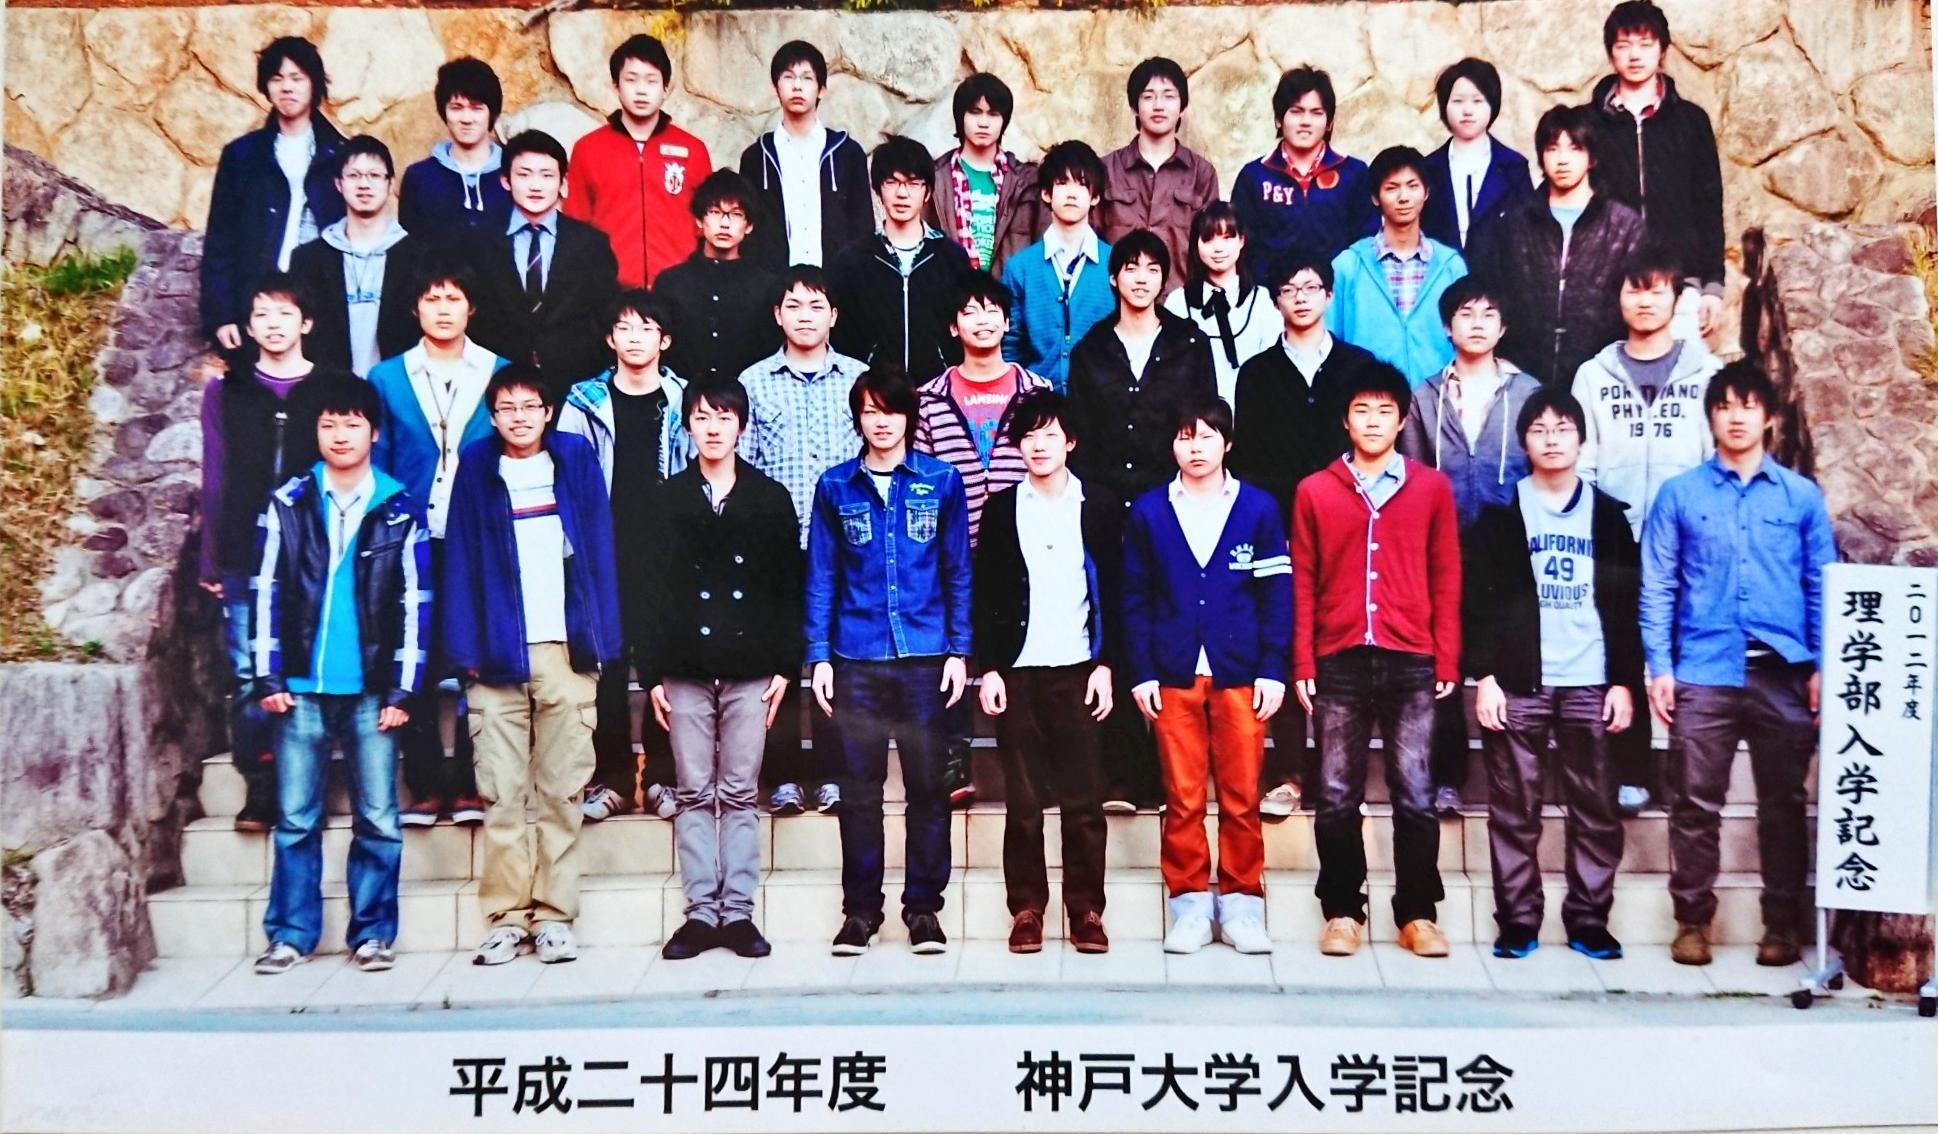
\includegraphics[width=0.8\textwidth]{./section/Kawori/figures/H24Nyugakushiki.jpg}
  \caption{最前列最左端に位置するのが我らのオガワマンであり、その左斜め上に(ポ)が君臨する。マタチチ大先生は最後列右から三番目に存在する。}
\label{fig:H24Nyugakushiki}
\end{figure}

その「カヲリ内部隠遁時代」から3年が経過したタイミングで、入学式を再現しようとする試みが見られた(図\ref{fig:H24NyugakushikiDummy})。
この入学式再現VTRは、後々まで参考にされる非常に重要な実験であり、その実験目的は、一つにはオガワカヲリの存在を明らかにしたい竹田側の意向があったことが知られている。
そのため、まだこの段階でも竹田・又吉はオガワカヲリの存在を知ることはなかったようである。

\begin{figure}[H]
  \centering
  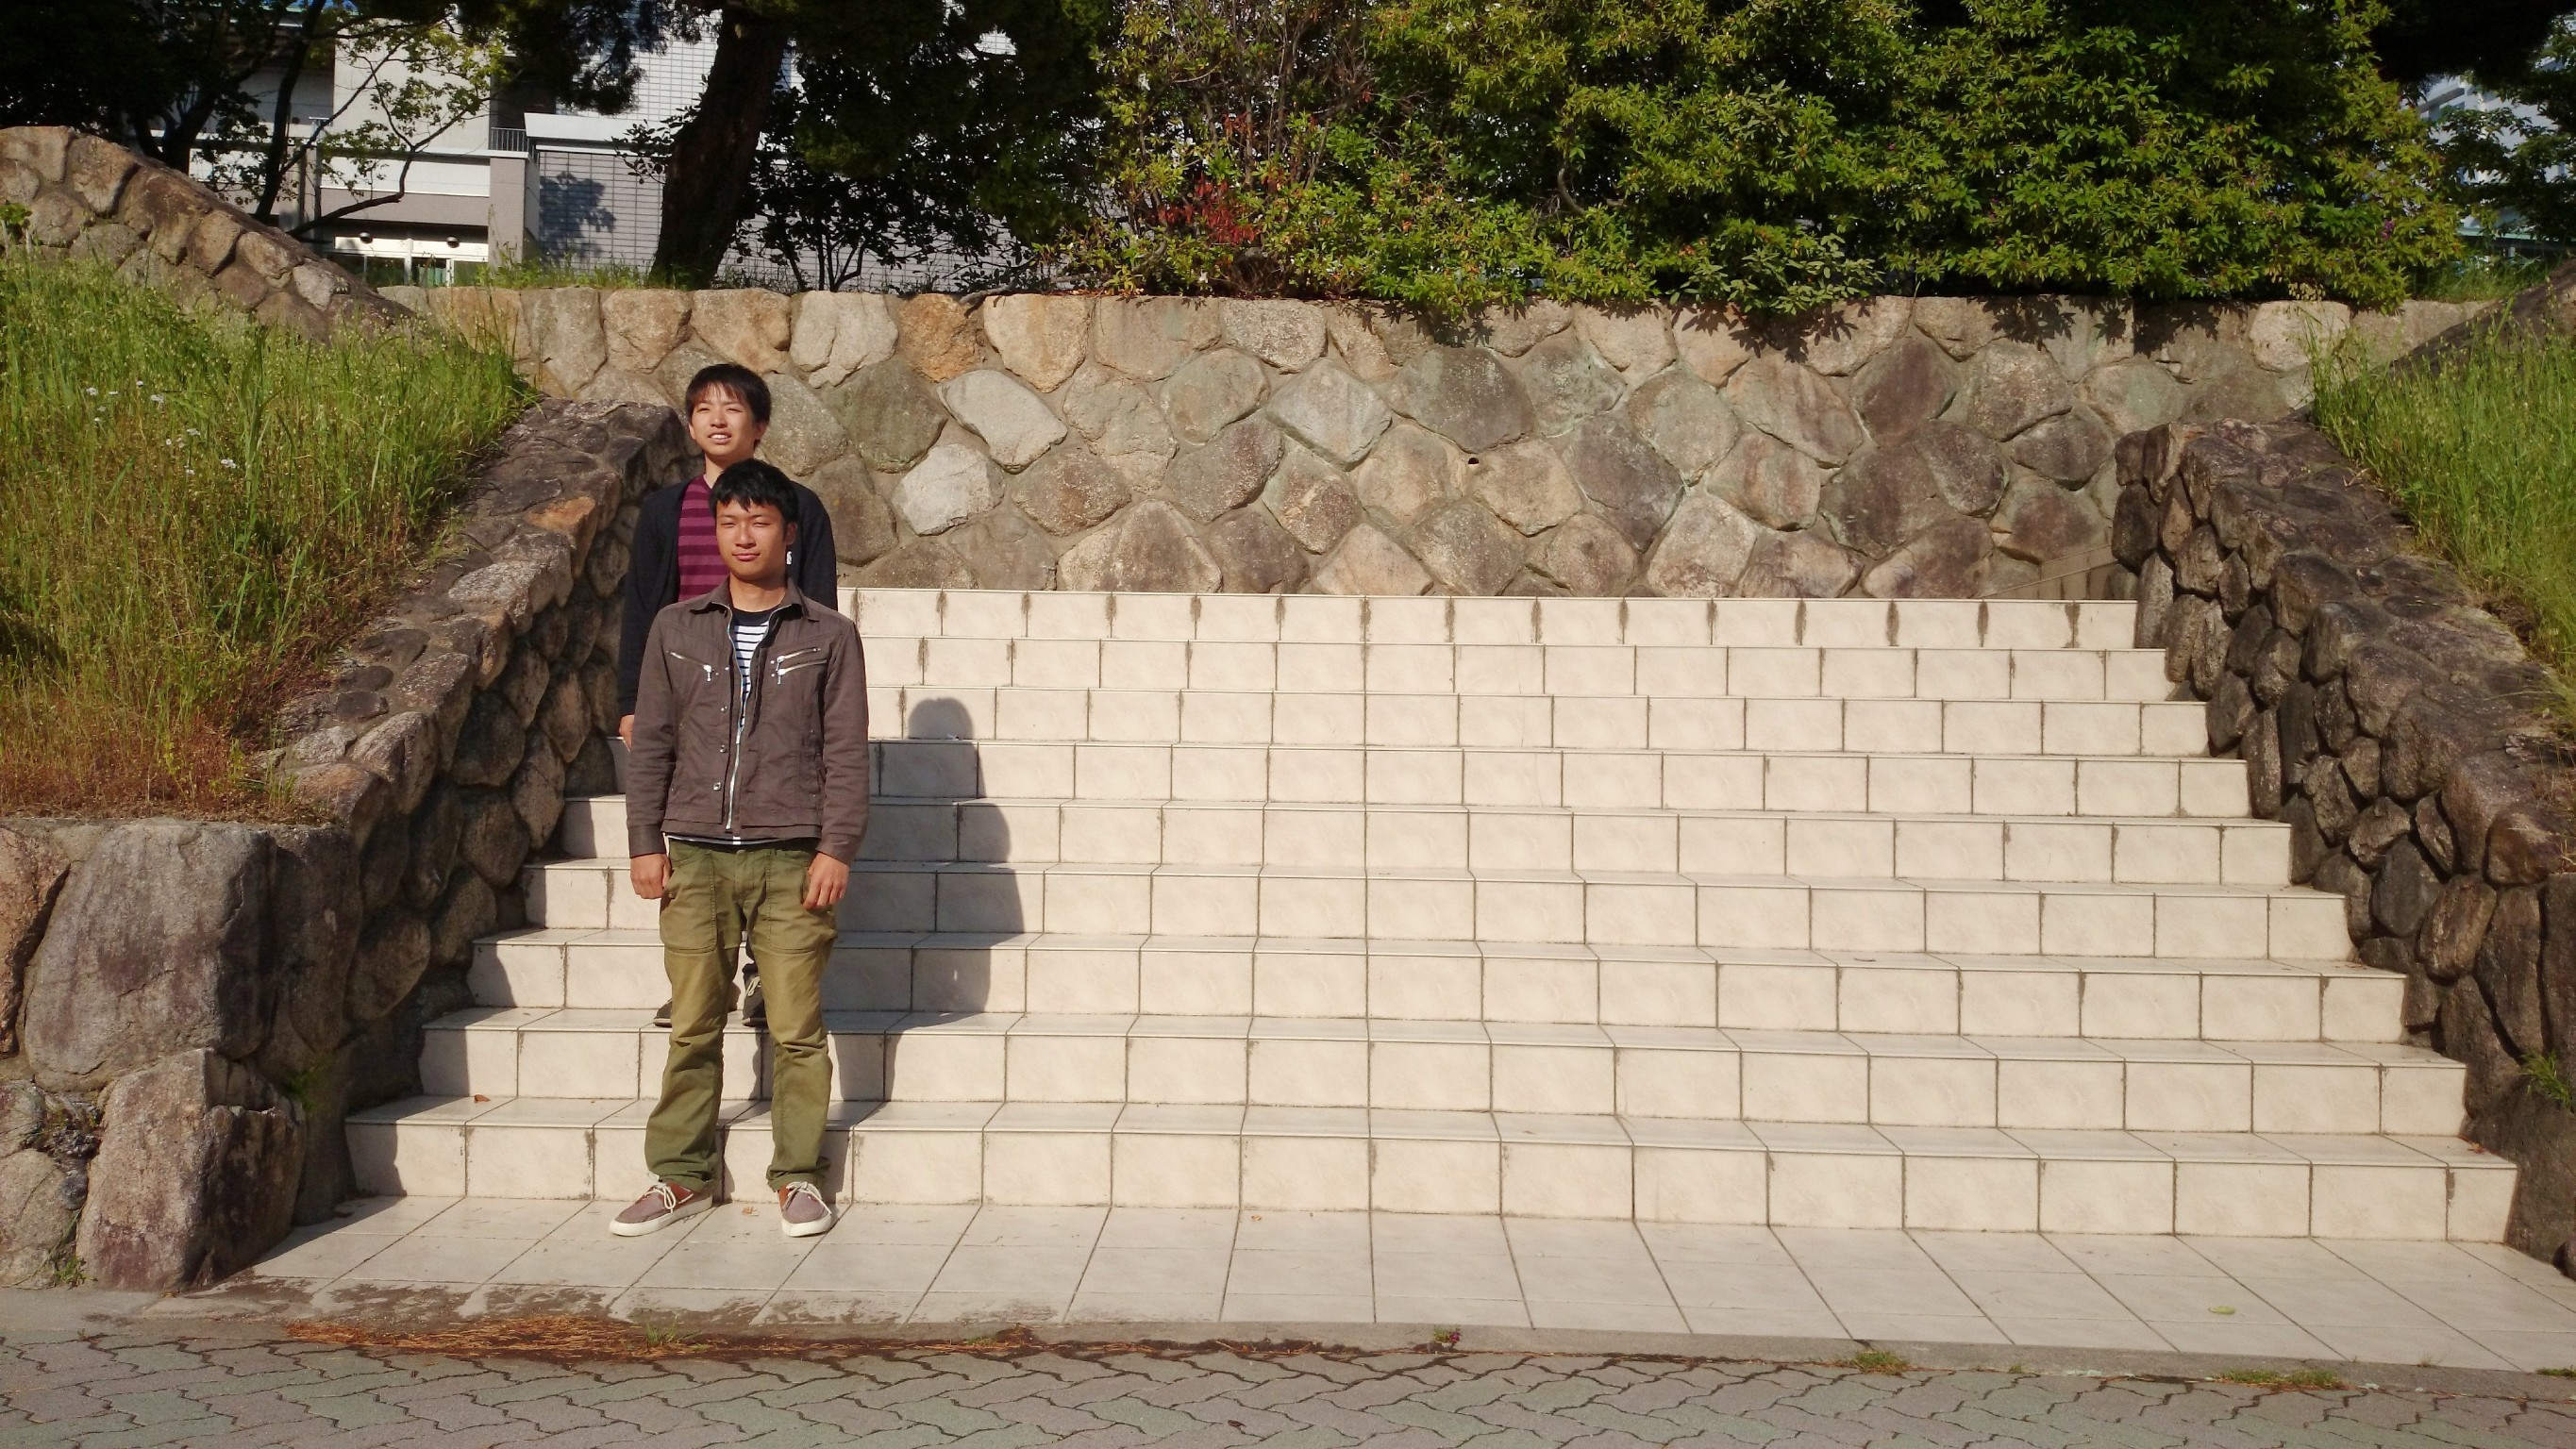
\includegraphics[width=0.8\textwidth]{./section/Kawori/figures/H24NyugakushikiDummy.jpg}
  \caption{最前列最左端に位置するのが我らのオガワマンであるが、しかし入学式の完全再現には至ることはなかった。図\ref{fig:H24Nyugakushiki}と見比べてもらえれば分かる通り、
  オガワマンの立ち位置がタイル一個分ずれてしまっているのである。}
\label{fig:H24NyugakushikiDummy}
\end{figure}

また、入学式再現の後に、入学式爆発実験も行った。
その実験結果を図\ref{fig:H24NyugakushikiDummyAbareru}に示す。
これから分かるように、入学式集合写真を撮影するタイミングで爆発が起きた場合は、人間はこの様に宙を舞うのである。

\begin{figure}[H]
  \centering
  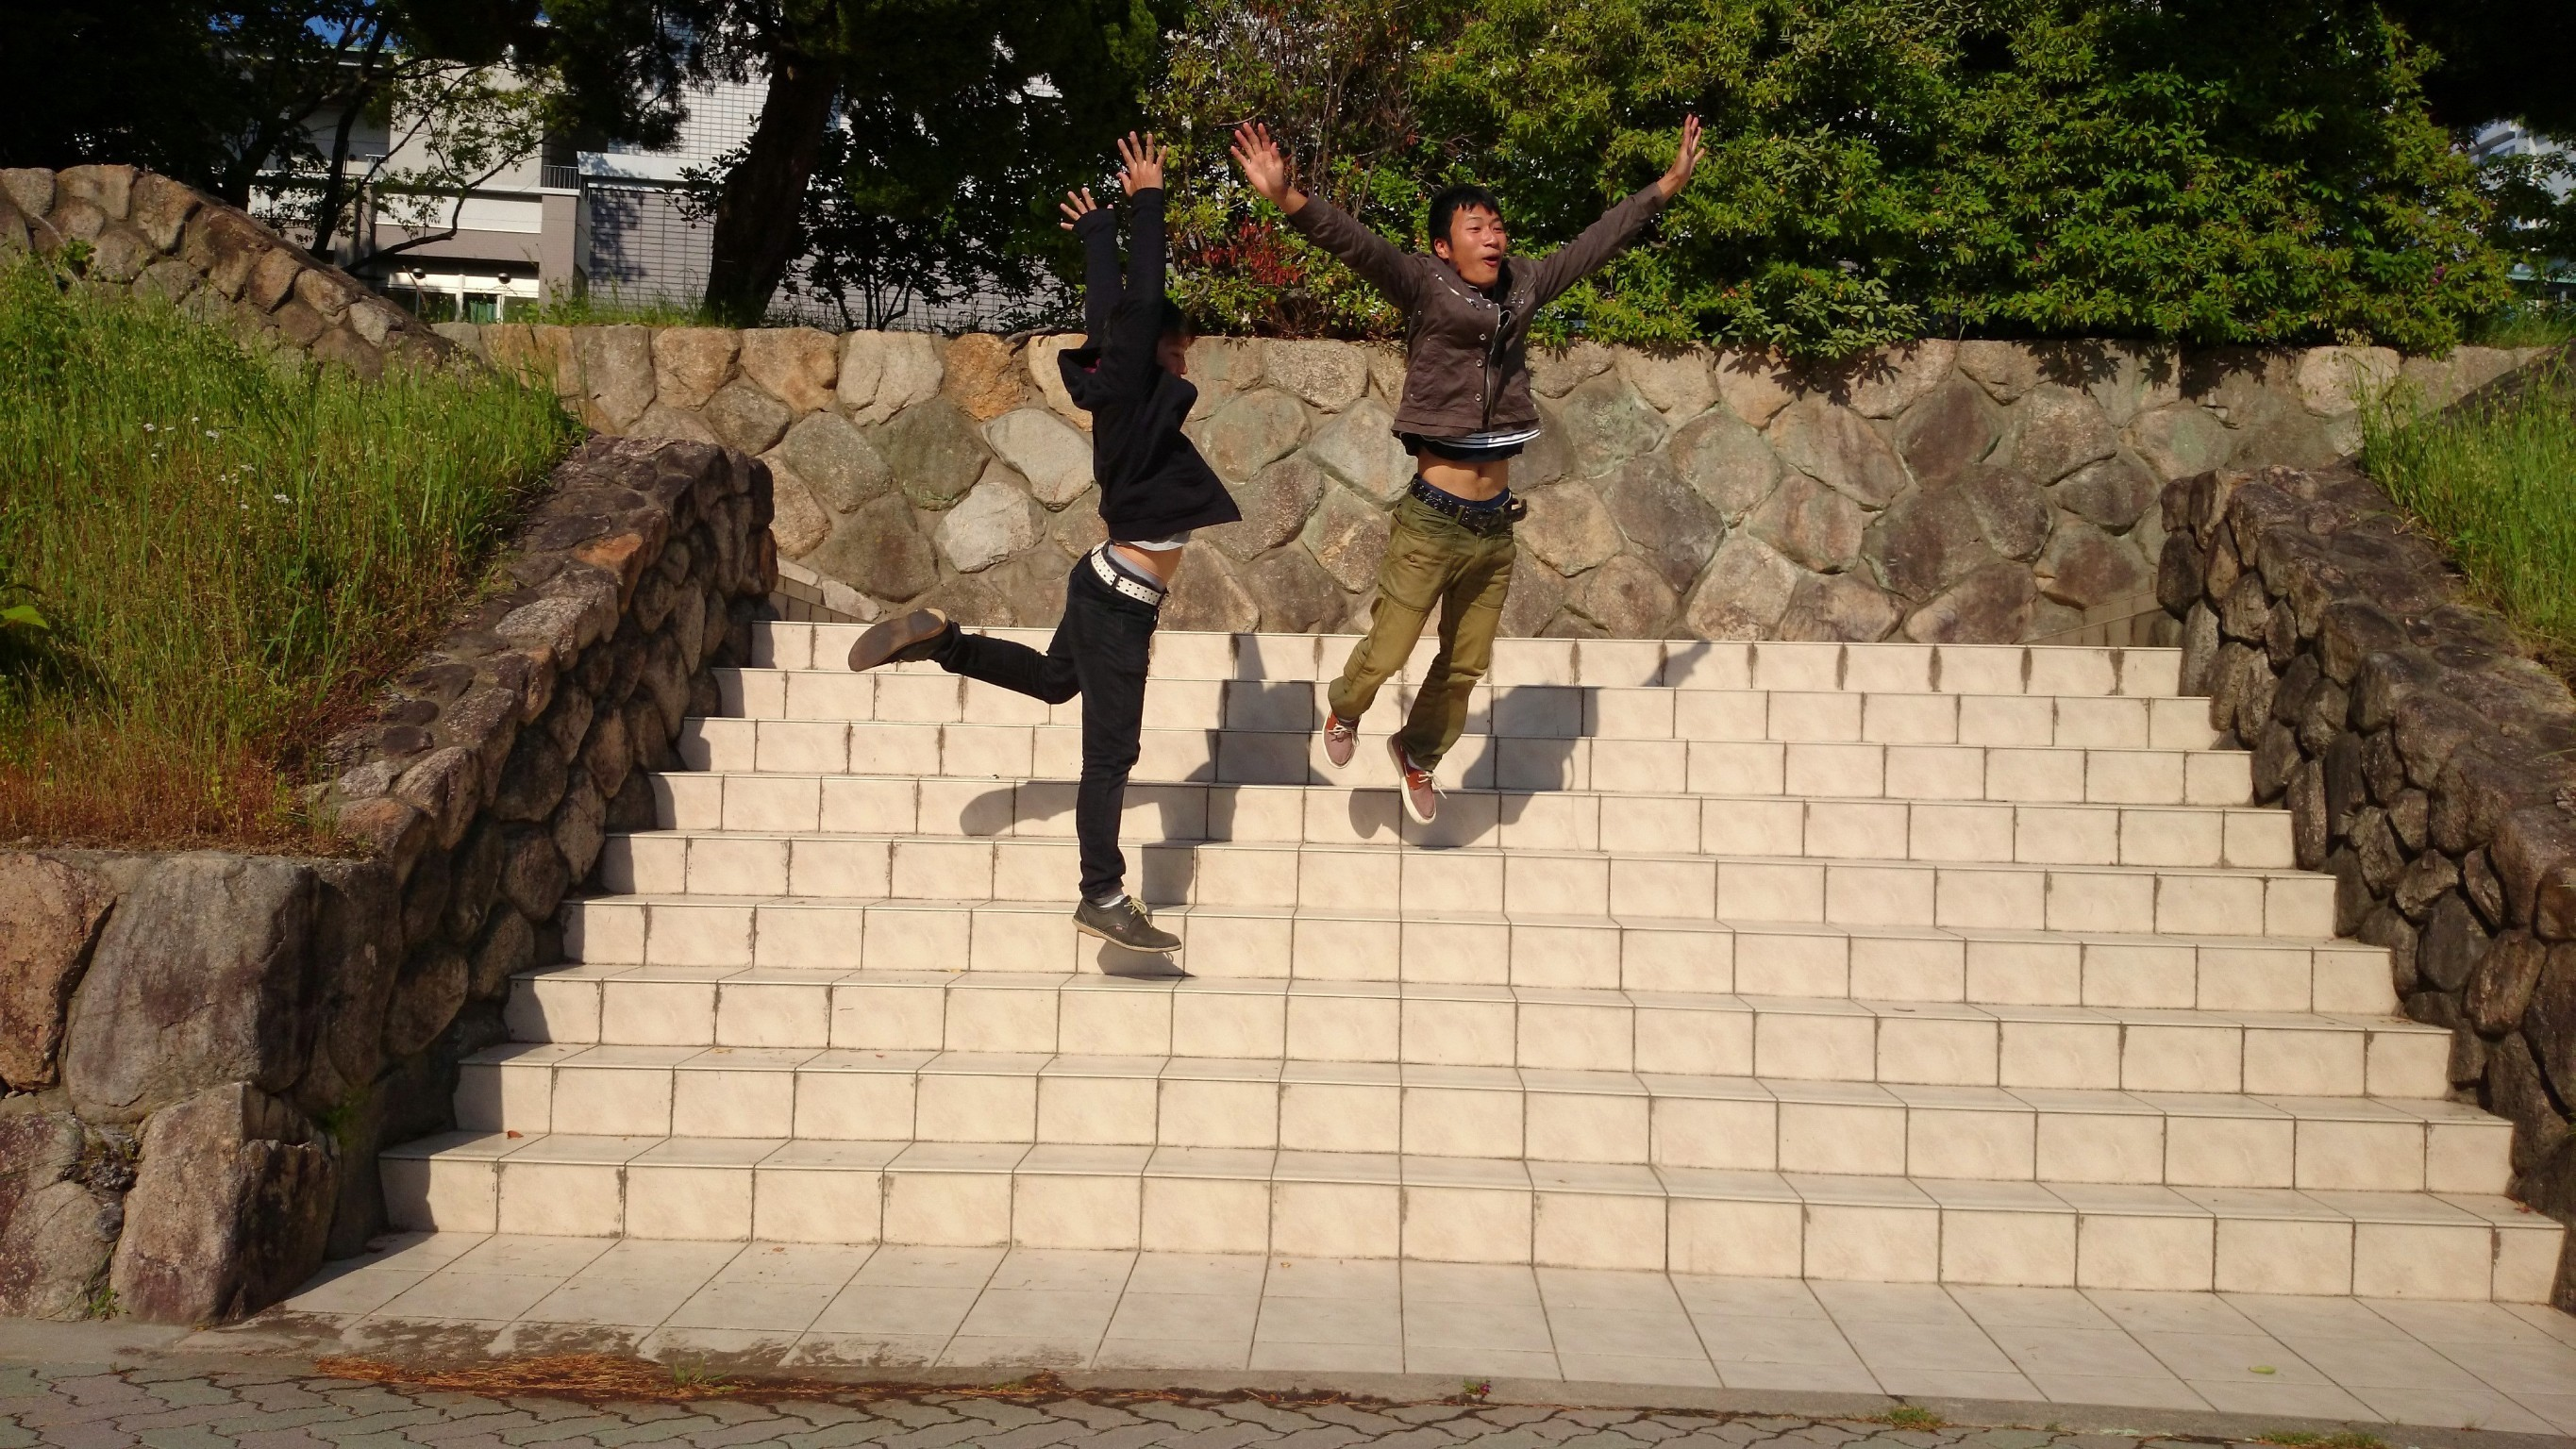
\includegraphics[width=0.8\textwidth]{./section/Kawori/figures/H24NyugakushikiDummyAbareru.jpg}
  \caption{入学式集合写真爆発実験。宙を舞う二人の姿が鮮明に記録されている。}
\label{fig:H24NyugakushikiDummyAbareru}
\end{figure}

\subsection{修士課程入学式}

また、我々が修士課程に入学した段階での写真を図\ref{fig:H28Nyugakushiki}に示す。
竹田・又吉の表情を解析すると、この時点ではオガワカヲリの概念はほとんど固定されていることが分かる。
その存在を強く認識してはいるものの、実際には面会したことがないために、概念としてしか理解できていない苦痛も見て取れる。
この時点ではカヲリという概念は、高度に抽象化された概念であり、その実体をイメージすることは非常に困難であった。
この苦痛が解消され、カヲリという概念が実在する象徴としての存在に昇華するまでにこの時点からさらに二年を要したのである。\par

\begin{figure}[H]
  \centering
  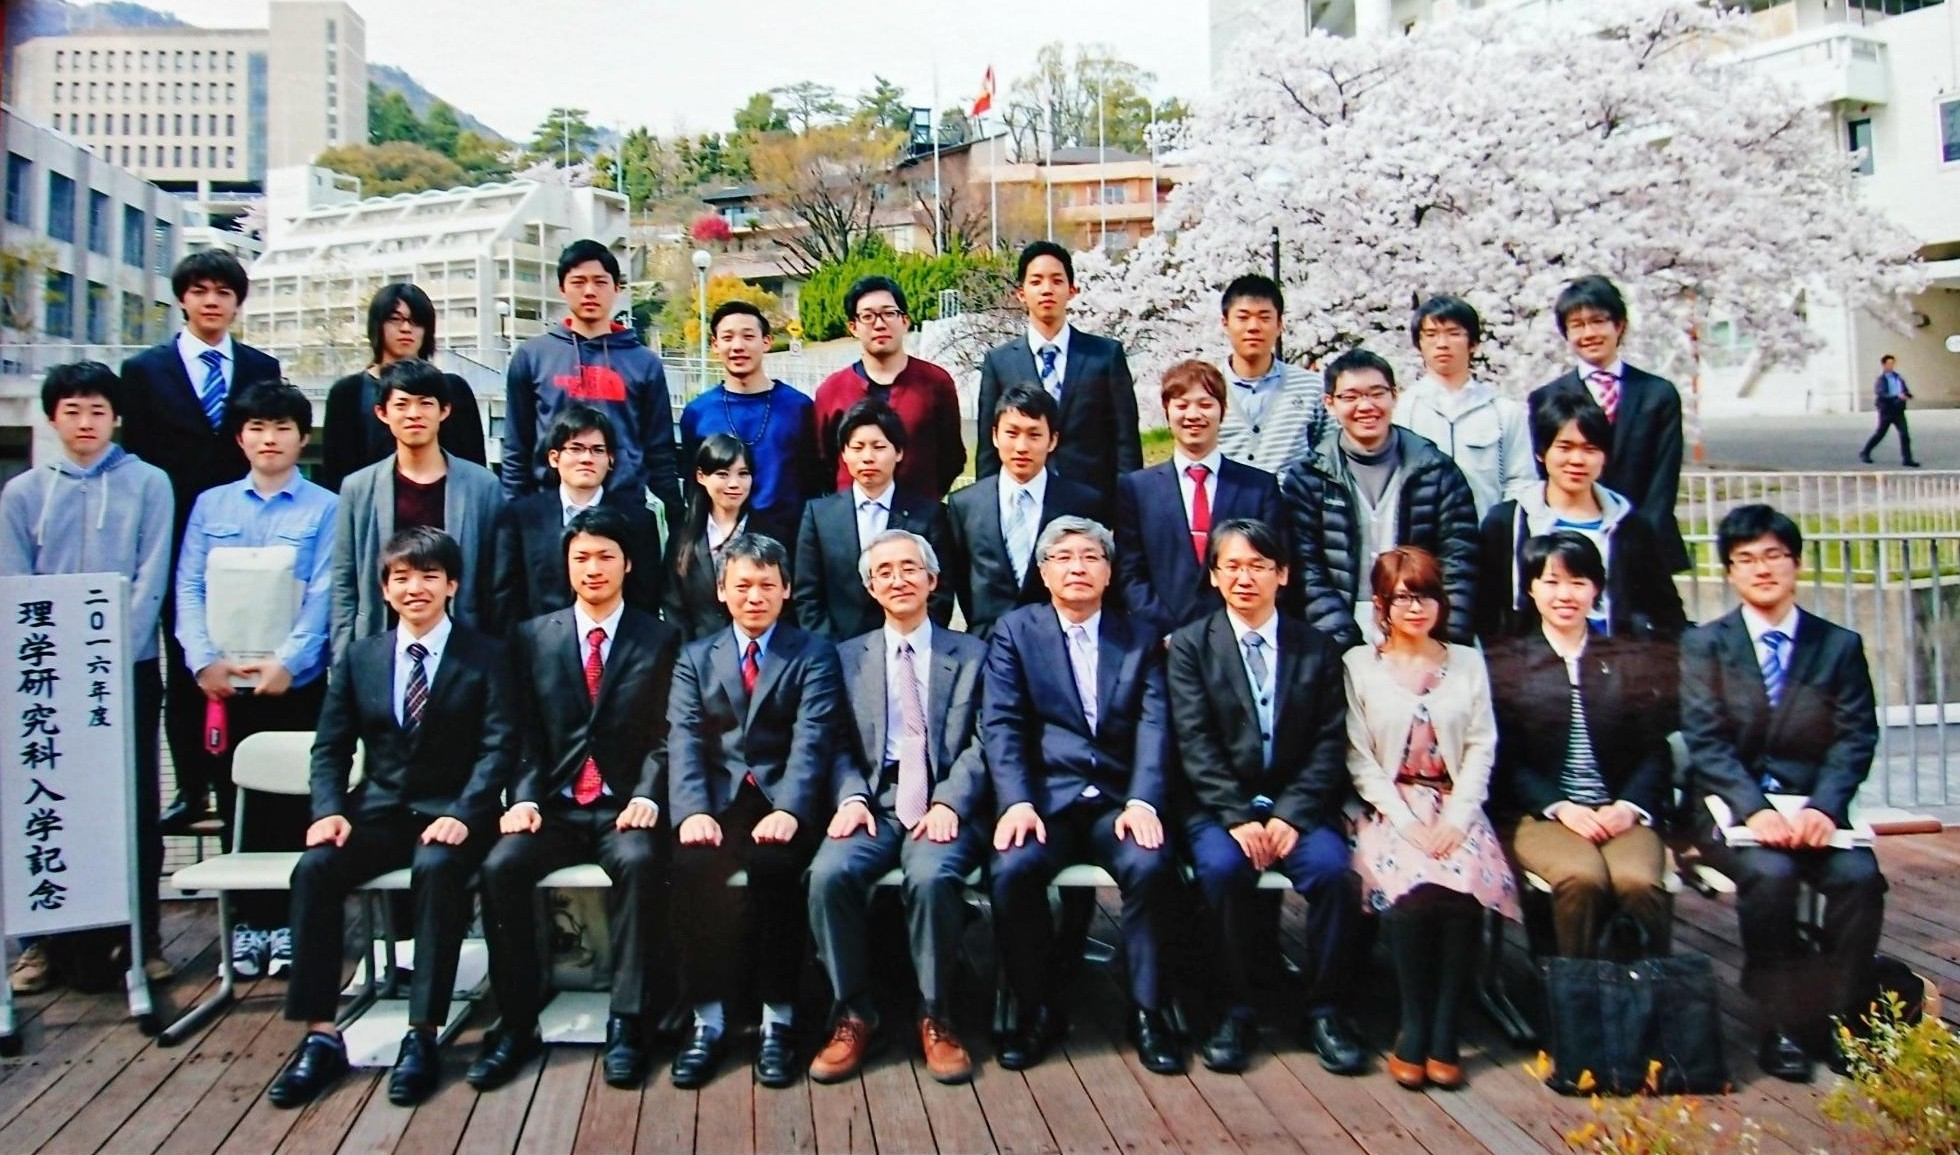
\includegraphics[width=0.8\textwidth]{./section/Kawori/figures/H28Nyugakushiki.jpg}
  \caption{2016年度理学研究科入学式集合写真。}
\label{fig:H28Nyugakushiki}
\end{figure}

\subsection{卒業式において}
以上までで、二種類の入学式について議論した。
それらの比較から、オガワカヲリの概念形成前後での竹田・又吉両名の表情の違いが容易に見て取れる。
また、この時点ではオガワカヲリは、聖なる母として粒子物理研究室のメンバーであれば誰でもその名を知っている存在であった。
これらから分かるようにオガワカヲリは非常に抽象化された、一種の宗教としての性質を持っていたことも心に留めておきたい。
何かに困ったとき、助けてくれるのはカヲリという概念を具象化したワードであり、「かをり、かをり」と続けざまに唱えることにより、
その場が凌げるという効能も持っていた。
\par
そのカヲリであるが、ついに修士課程卒業式のタイミングで、神戸に降臨するとの情報をキャッチすることができた。
今までは概念上の存在であり、オコワを京都から神戸へ運搬していた人物としてしか具体的な情報を持っていなかった我々であるが、ついにその実在化に向け運命の歯車が回り始めたのである。
\par
図\ref{fig:OgawaManKawori}を見ていただきたい。
非常に微笑ましく、我々が入学以来六年間追いかけ続けたカヲリという概念がついに、オガワマンの横で具象化した瞬間である。
写真の女性がカヲリ本人であり、オガワマンをオコワマンとして仕立てていた女性であるのだ。

\begin{figure}[H]
  \centering
  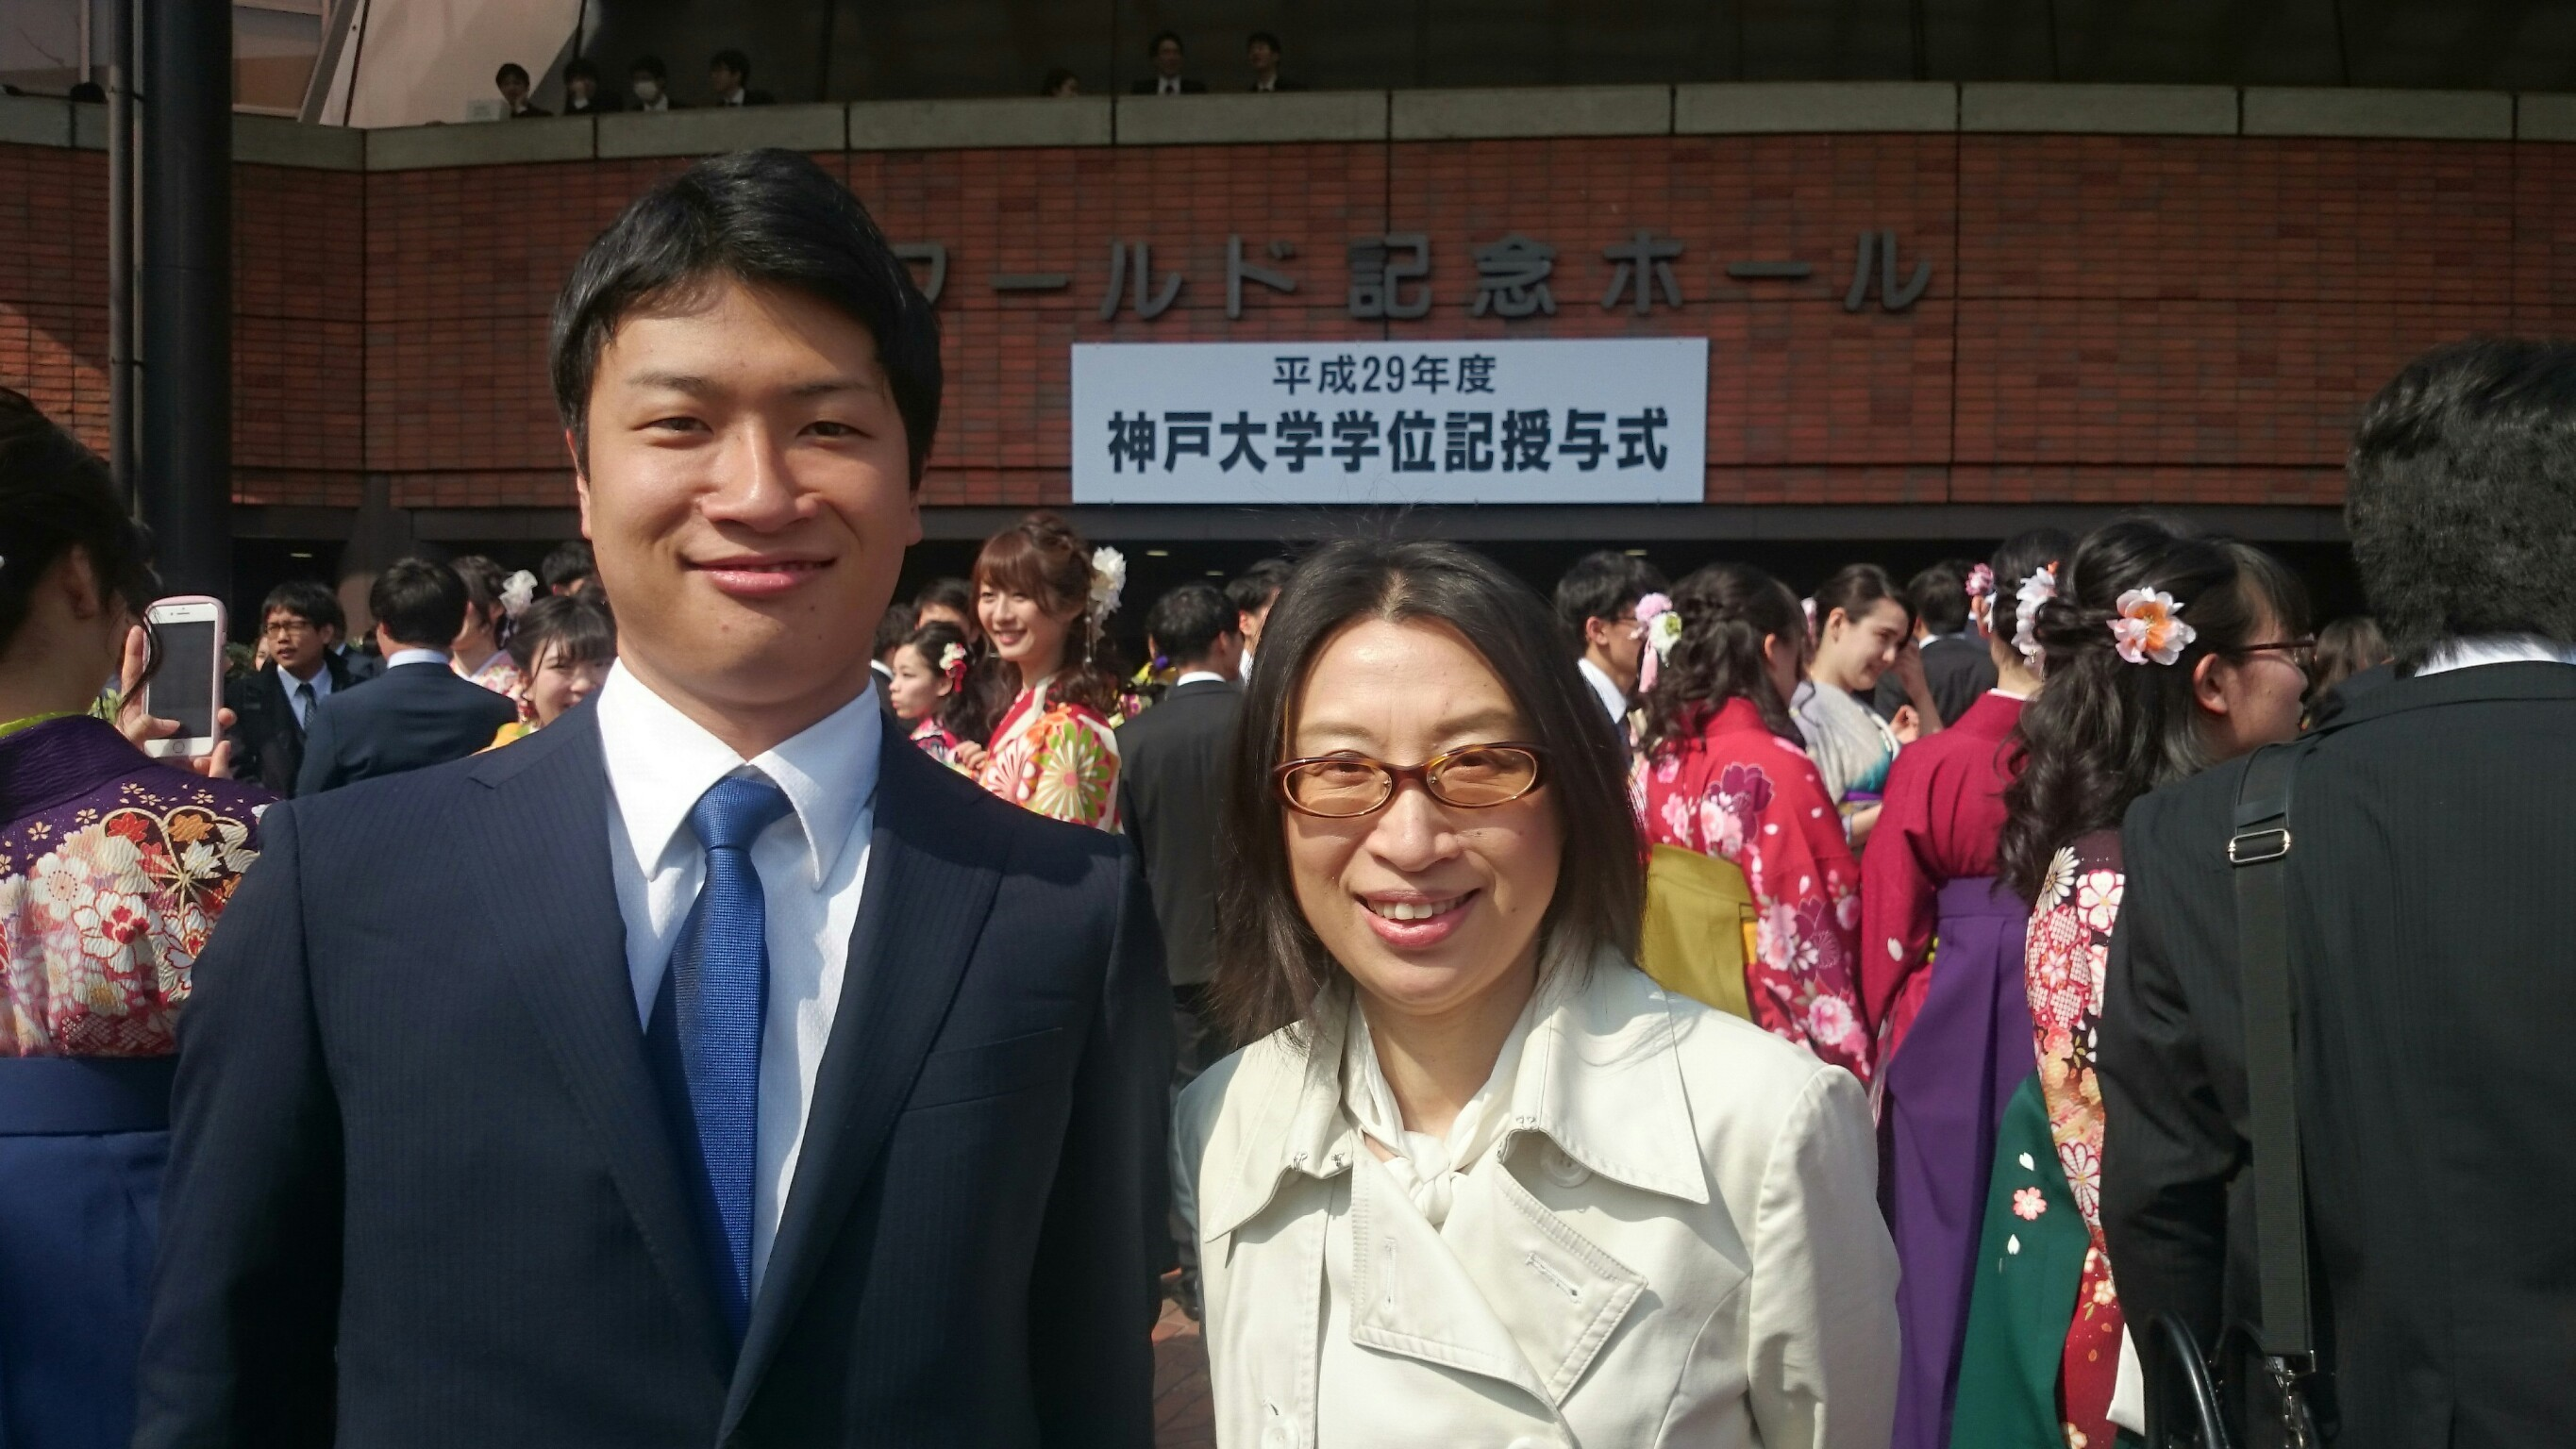
\includegraphics[width=0.8\textwidth]{./section/Kawori/figures/OgawaManKawori.jpg}
  \caption{小川圭将と小川かをりとの夢の共演である。}
\label{fig:OgawaManKawori}
\end{figure}

\par
さらに竹田・又吉両名に加え、粒子物理研究室随一のチャラ男若宮光太郎との、2ショットにも笑顔で答えてくれたのである。
図\ref{fig:KaworiMatayo},\ref{fig:KaworiPo},\ref{fig:KaworiPika}に示す。

\begin{figure}[H]
  \centering
  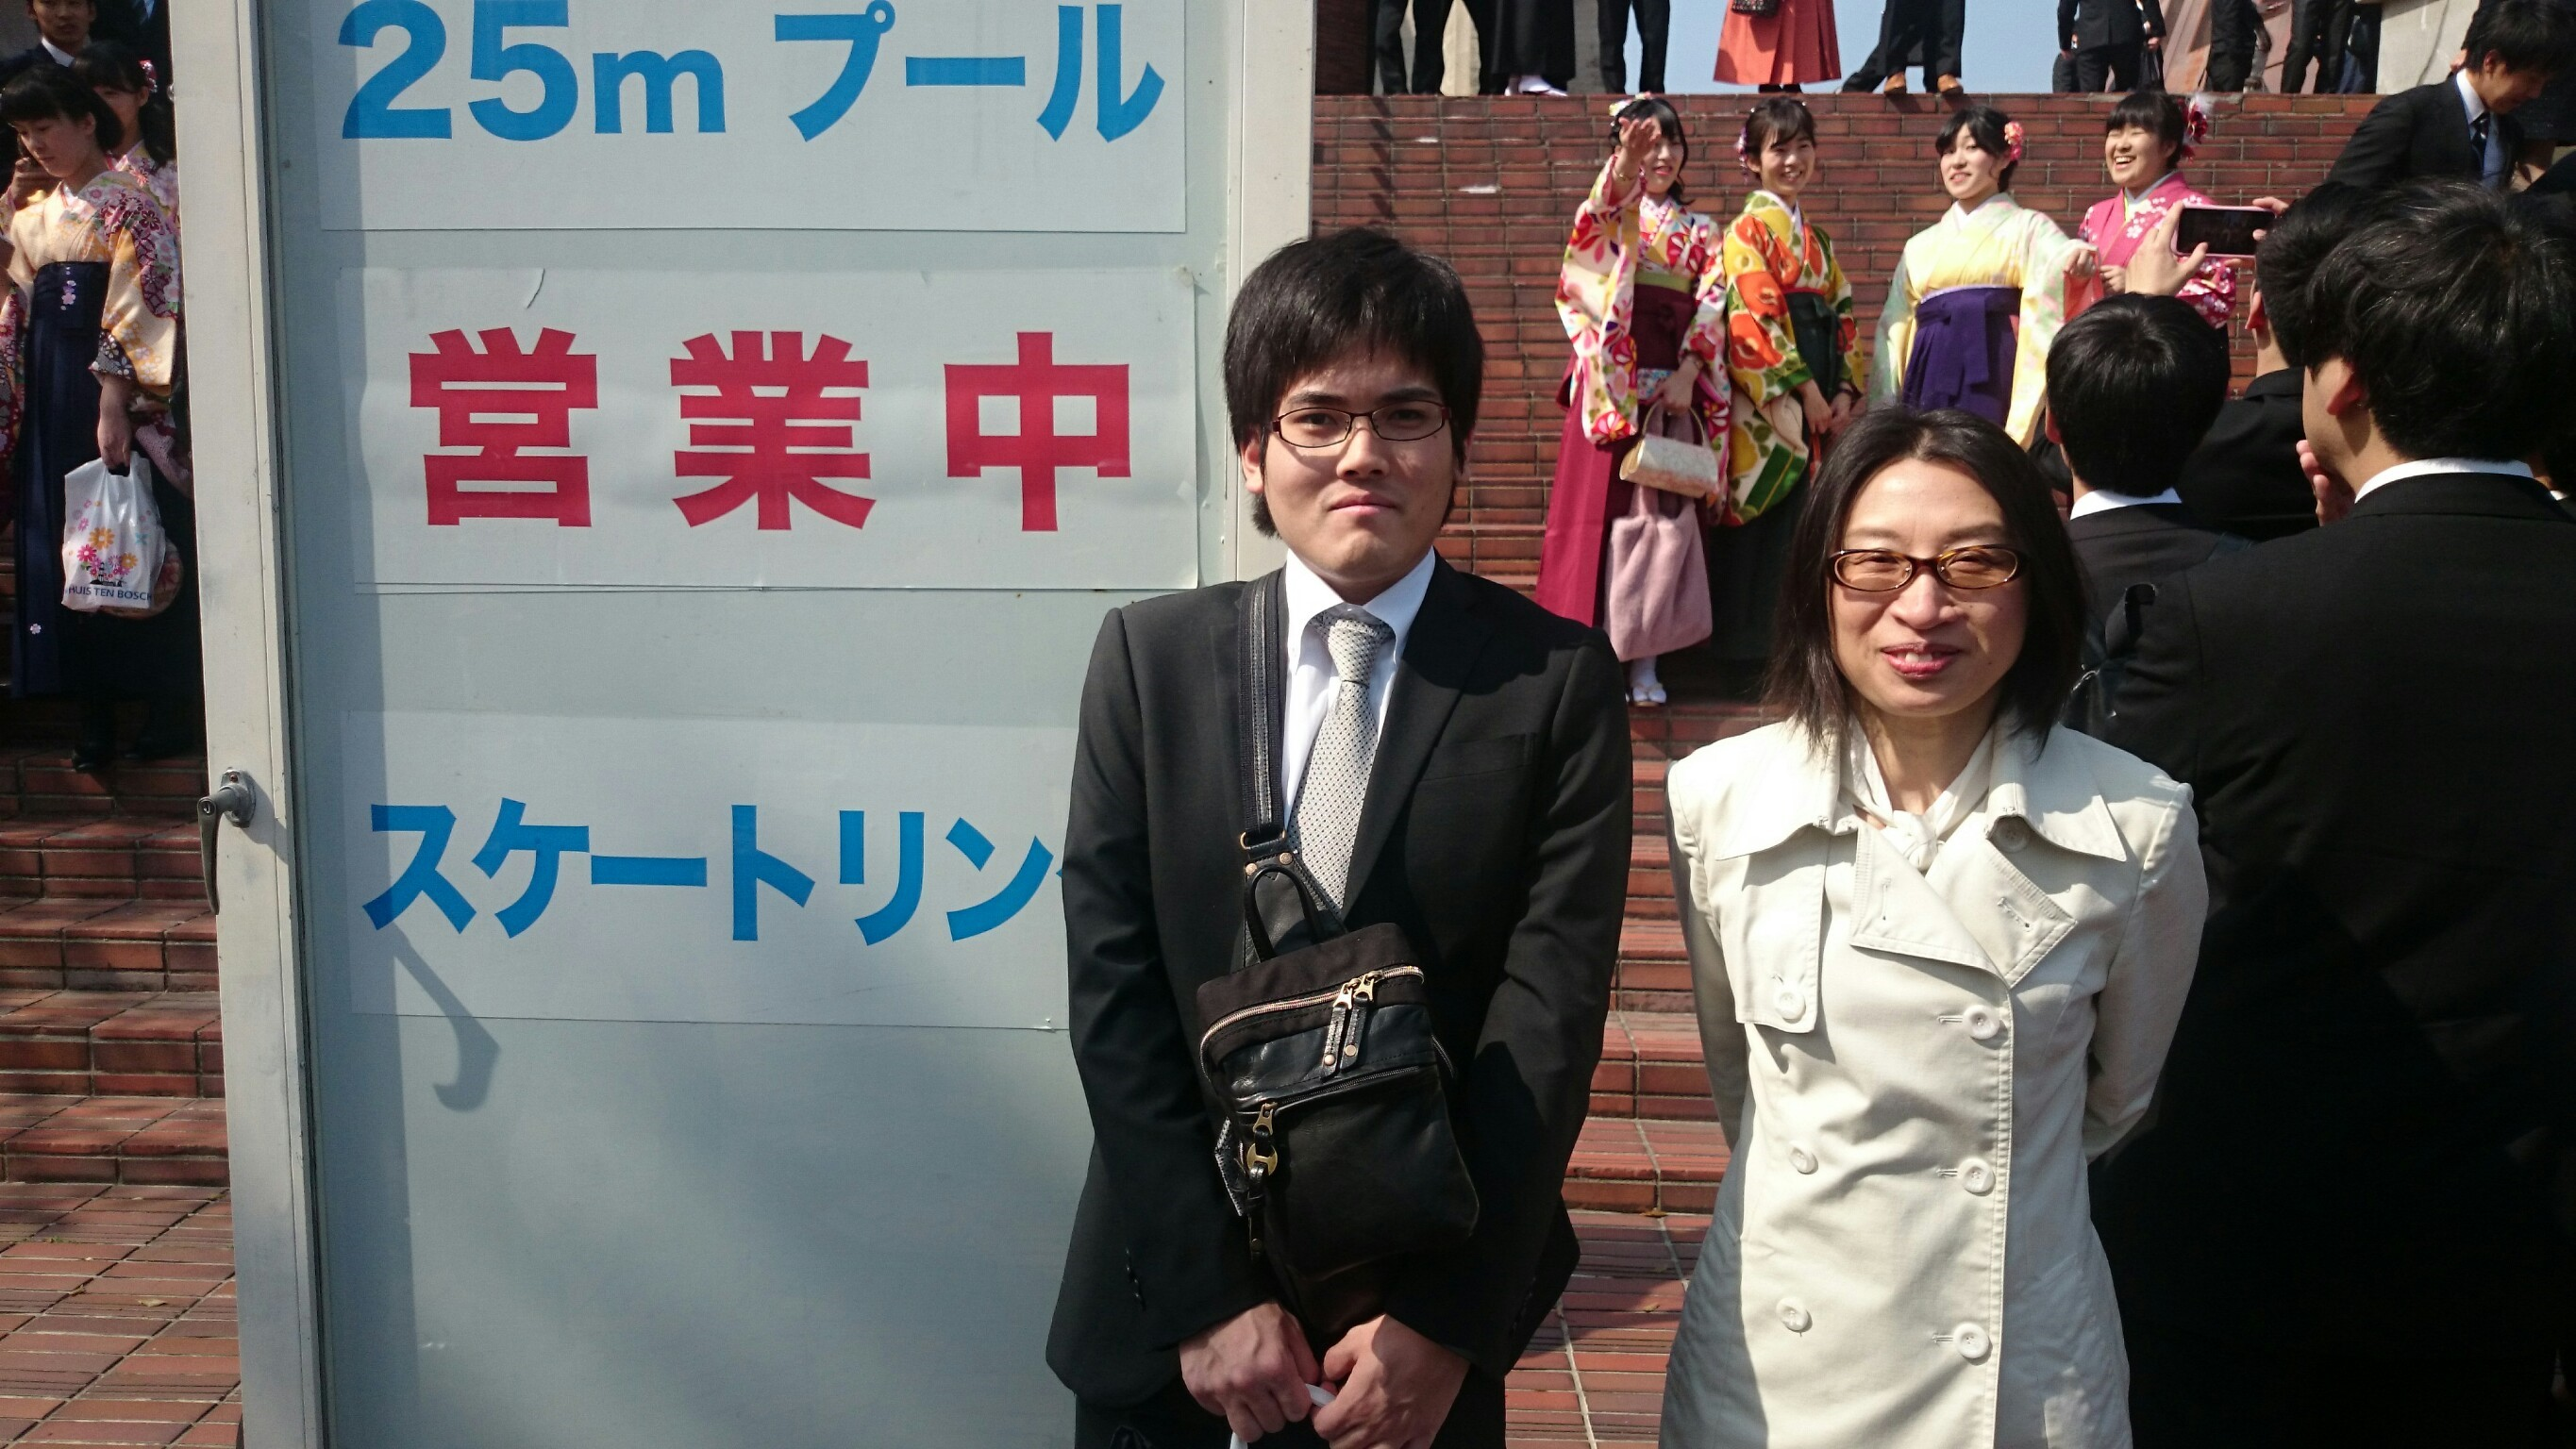
\includegraphics[width=0.8\textwidth]{./section/Kawori/figures/KaworiMatayo.jpg}
  \caption{又吉清掃員とかをり氏との記念写真。
  何を隠そう、このプールは竹田氏思い出のプールなのである。
  たまに泳ぎに来ていたのである。
  又吉清掃員もまた、高校時代には水泳部という主張をしており、本プールは非常に想い出深い場所であり、
  その場所において伝説の写真が撮影されたわけである。}
\label{fig:KaworiMatayo}
\end{figure}

\begin{figure}[H]
  \centering
  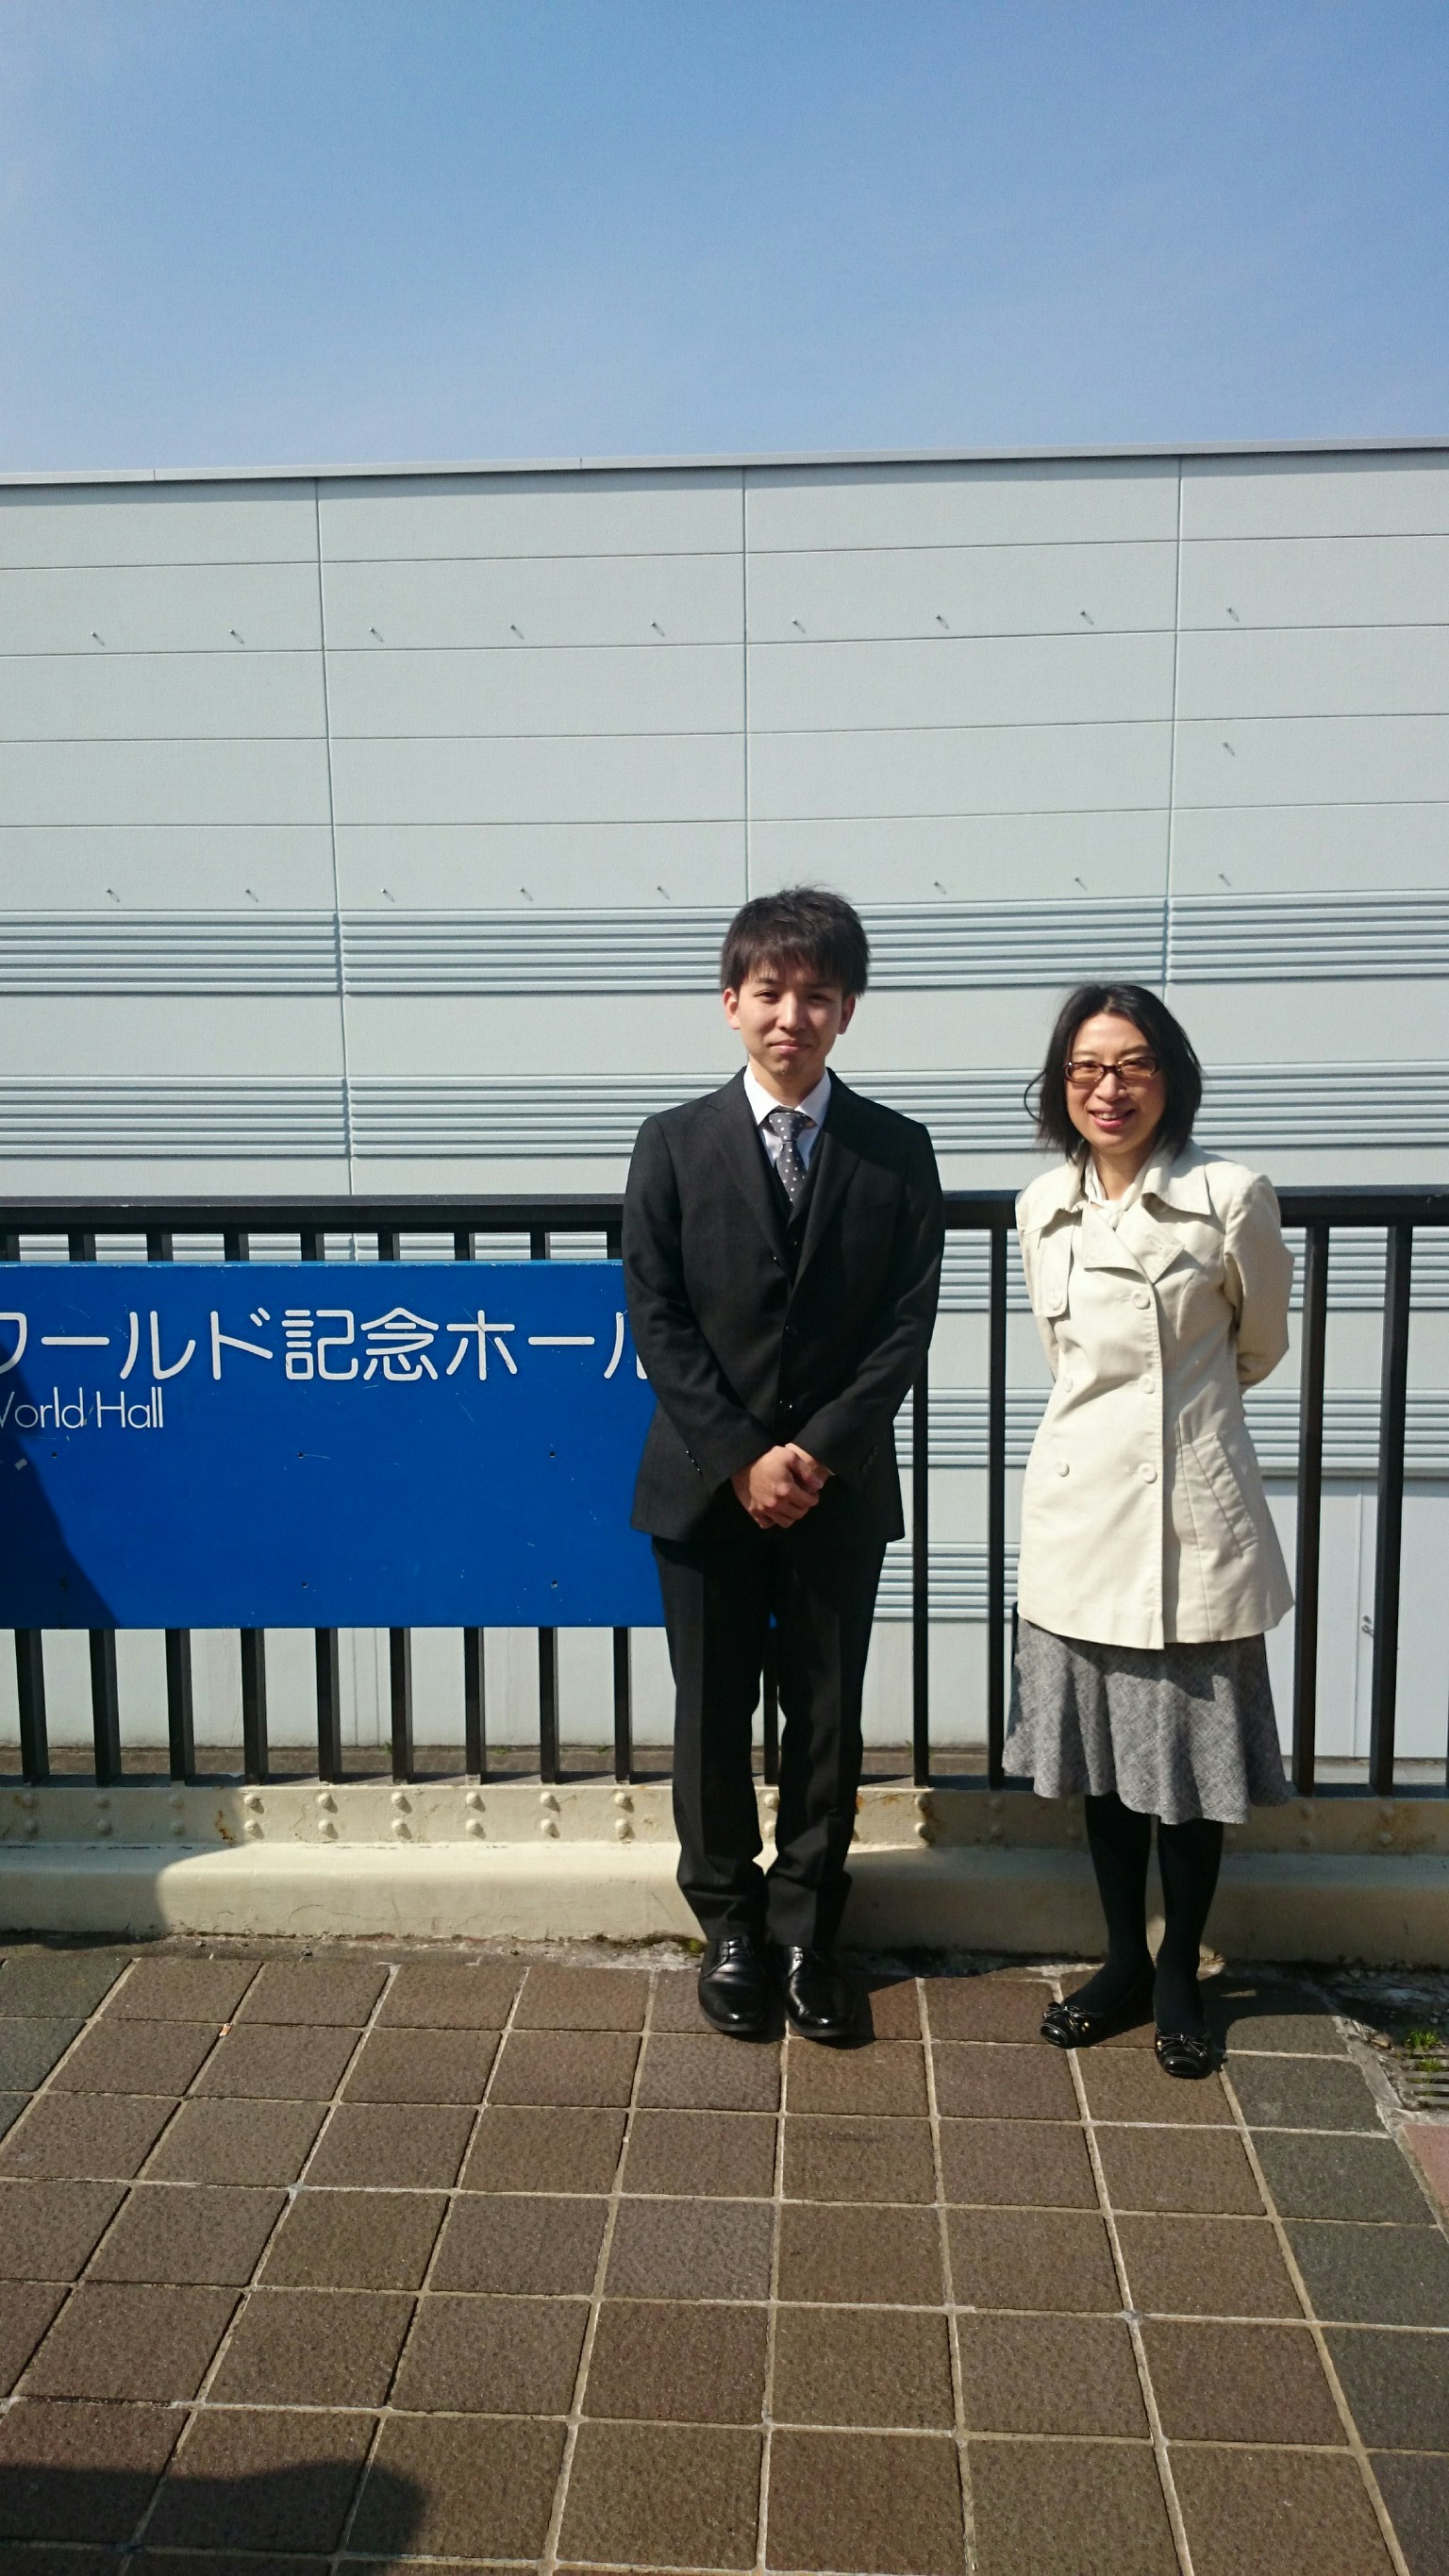
\includegraphics[width=0.5\textwidth]{./section/Kawori/figures/KaworiPo.jpg}
  \caption{かをり概念拡散部隊隊長である竹田氏と、かをり氏との直接対決を記録した記念すべき一枚。
  修士課程卒業には竹田氏の親族は出席していないため、かをり氏の粋な図らいにより竹田母の代役を努めて頂いている。
竹田隊長は日光が眩しいのか、照れくさいのか、それとも今までイジり倒してきた相手をいざ目の前にして半笑いなのか分からないが、その評定はどことなく微笑んでいる。
それに対してかをりは、口角をぐっと上げ、余裕の笑みを浮かべている。
しかし、後ろに回した手は、いついかなるときでも竹田氏を倒すだけの用意ができているということであろうか?\\
どちらかと言えば、この写真の最重要ポイントはポートライナーの駅を出て徒歩10歩の場所で、人通りがものすごくあるドリル目線の環境で撮影されたということであろう。
端から見れば親子写真を撮っている様に感じられるのであろうが、その実全く関係のない二人を、そのかをりの息子が写真を撮っているのである。
もし仮に知り合いに「あの方はお母さん?」と聞かれた場合、返答の選択肢としては説明放棄しか存在しない。
  }
\label{fig:KaworiPo}
\end{figure}

\begin{figure}[H]
  \centering
  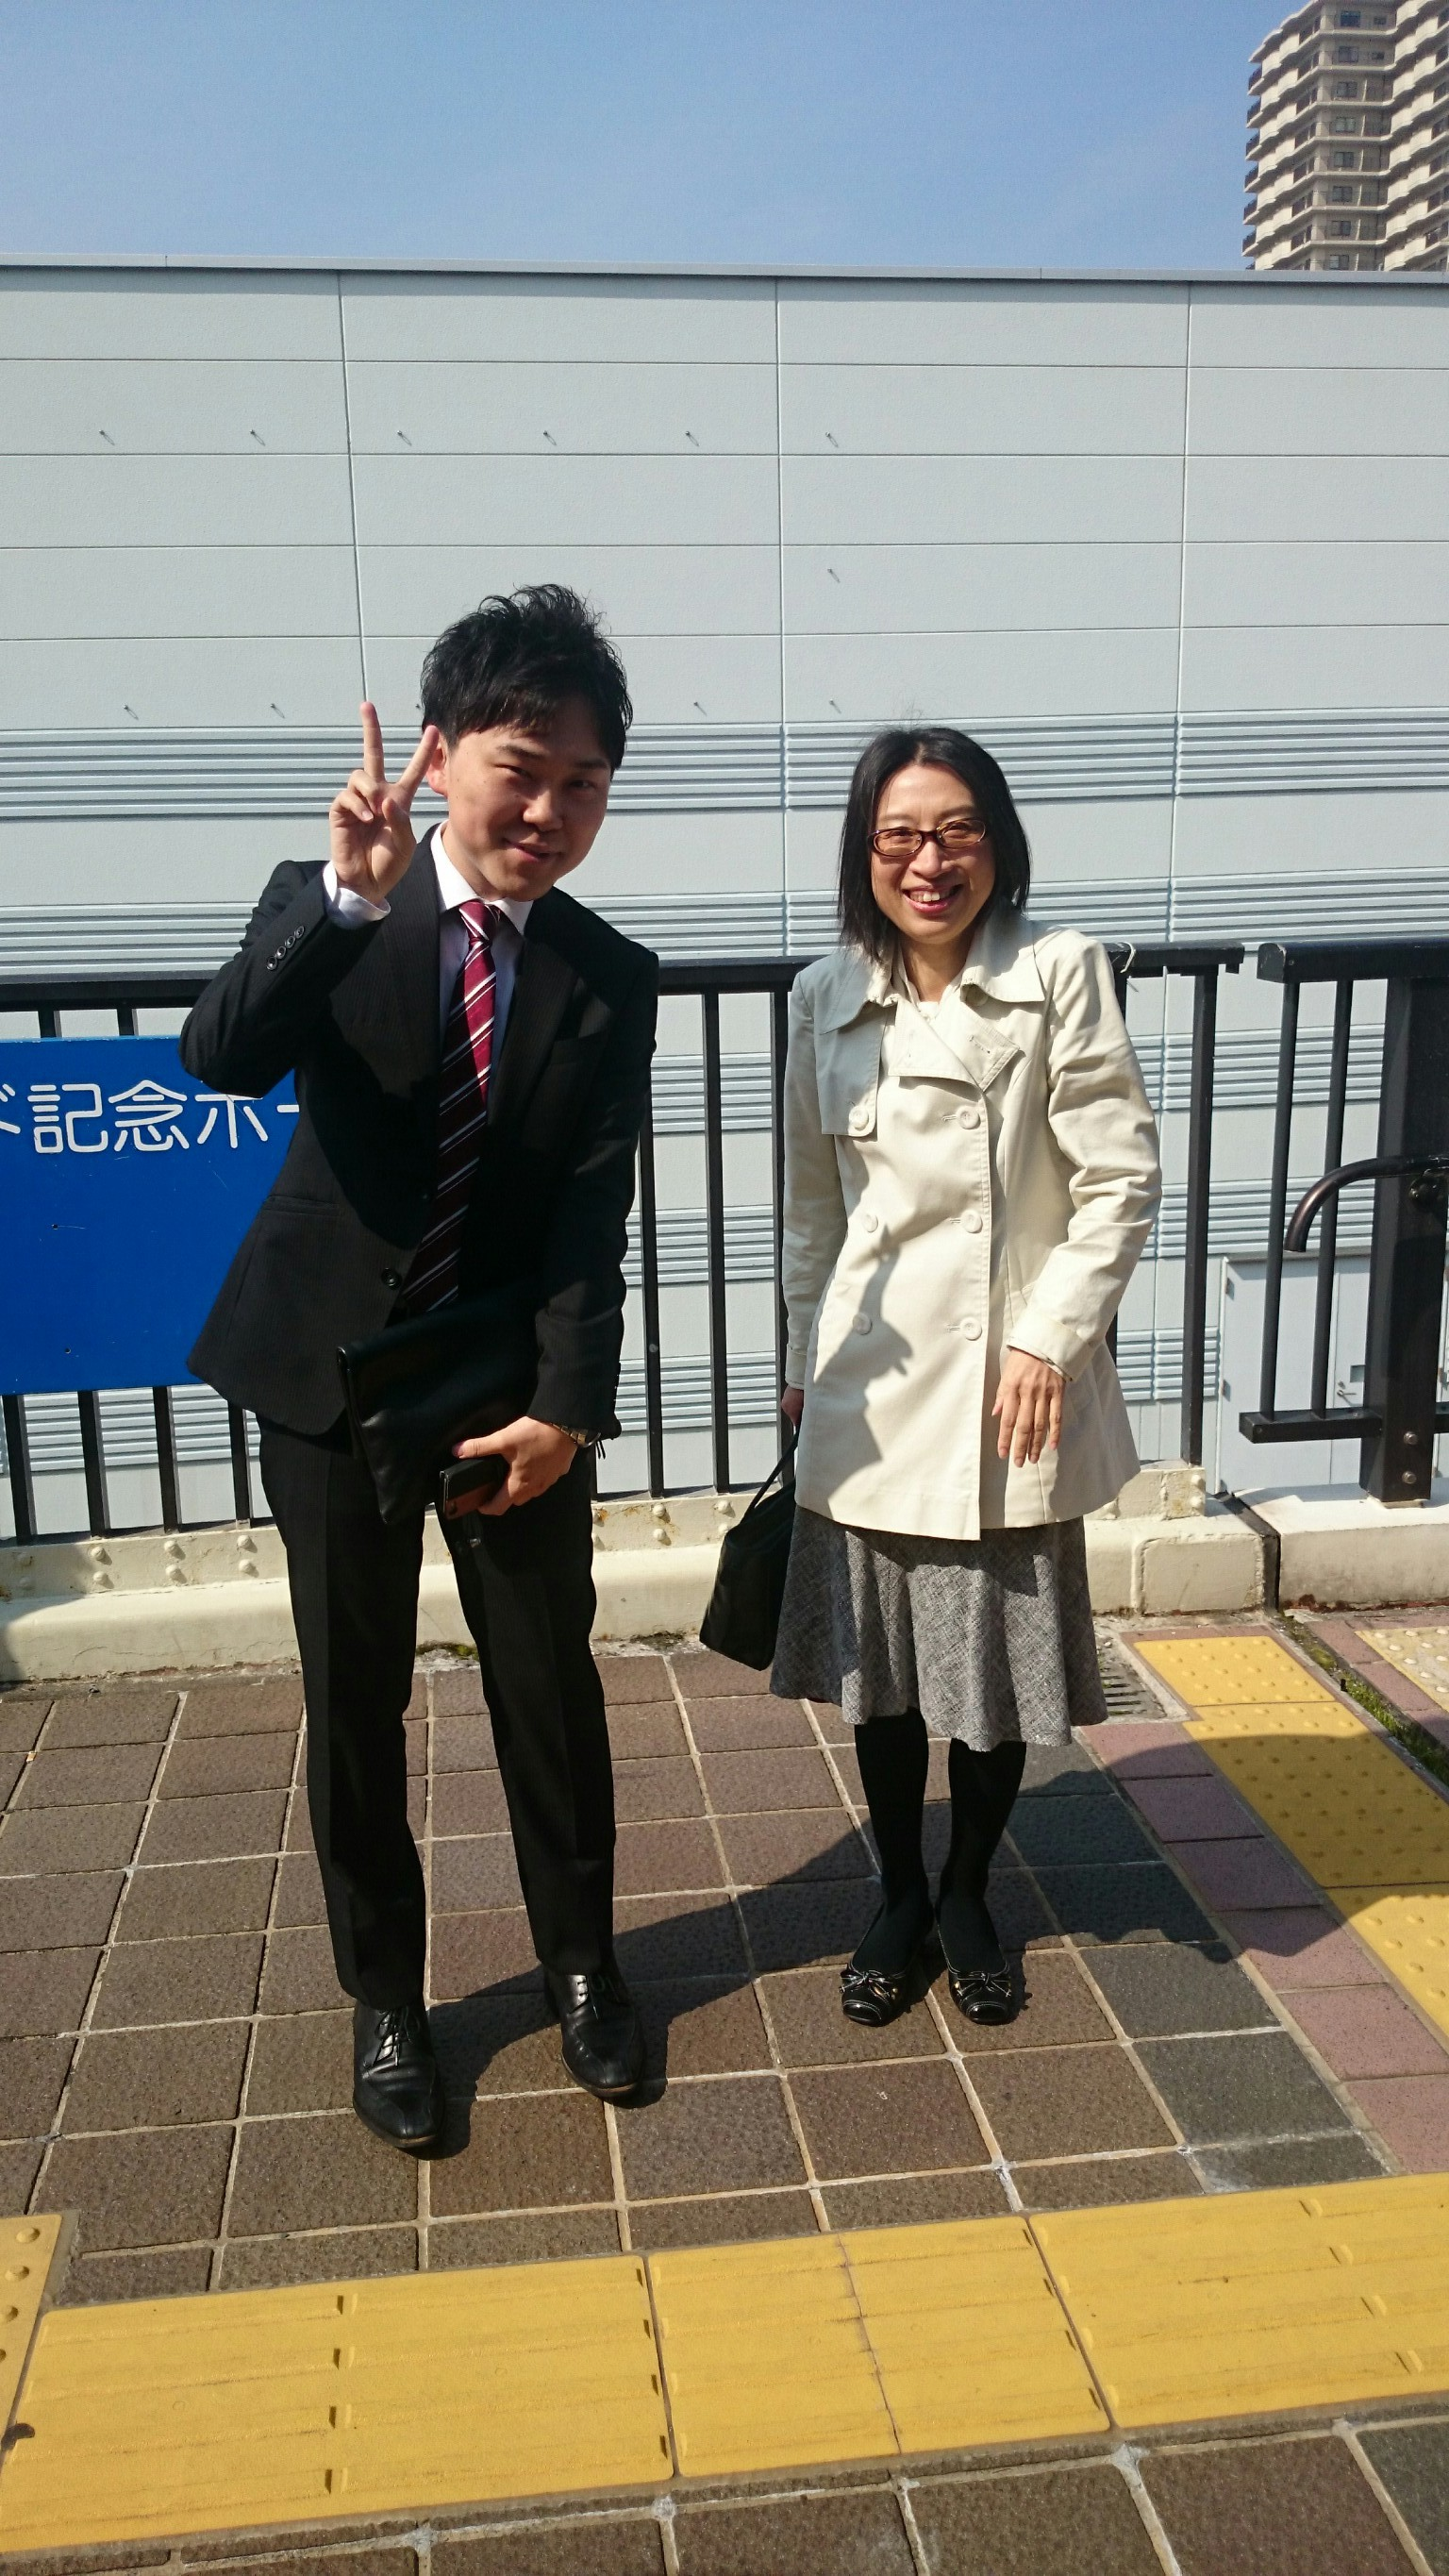
\includegraphics[width=0.5\textwidth]{./section/Kawori/figures/KaworiPika.jpg}
  \caption{チャラ男代表のミツ太郎と、かをり氏の直接対決。図\ref{fig:KaworiPo}との違いは、そのチャラさであろう。
  明らかに写真のテーマが真面目さか、チャラさかに二分されるであろう。
  ミツ太郎氏はピースサインを決め、それに対してかをり氏は少し照れているのである。
  }
\label{fig:KaworiPika}
\end{figure}


\section{又吉先生による評価}
かをりの特筆すべき点はその「を」にあると私は考える。をという文字は現代では助詞の一つとしてしか使われないが、伝統的には「お」と同じ音を意味する格式の高い文字だ。その「を」を名前の真ん中に持ってくるということに高い気品を感じることができる。大変にありがたい文字列であるのだ。おみくじで言えば「かをり」は大吉に近い。これがもし「かおり」であったなら中吉か吉程度で止まっていたかもしれない。大吉と中吉は数字で表すと100と50くらいの違いだ。博多華丸と大吉くらいの違いがある。仮にパンで例えるならフランスパンとコッペパンほども異なっているのだ。
かをりという名前に込められた真の意味を私は知ることはできないが、推測するとすれば第一に思い浮かぶのが「香」だろうか。香は日本の古典にも多く出てくる言葉だ。良い匂いを意味するだけでなく、気配や予感といった雰囲気的なものも示すのが香だ。昔の人はより上質な香りを求めて様々な動植物、はては水や鉱物までも求めた。大変ありがたいものだったのだ。
しかしもし「かをり」の意味するところがそれではなかったならどうだろう。
かをりとは「かをり」なのか、「か」と「をり」なのか、もしや「かを」「り」なのか。先に述べたとおり、私はその真の意味を知ることはできない。
この文章を読んでいる方よ、どうか私に代わり、「かをり」の真の意味を明らかにしていただけないだろうか。それだけが私の最後の願いだ。

\section{結論}
ここまでで議論したカヲリという概念を締めくくるにふさわしい御言葉を、小川男葉集第五版から引用しておこう。
\begin{quote}
美容院には来週末で予定していたのでバサバサ頭が気になった(絵文字)。普段はもっと若々しくてハツラツとしてキレイにしてると友達に言っといてな
\end{quote}
我々は今後、カヲリ完全体を観測すべく、次世代の実験施設を建設する予定である。
